%----------------------------------------------------------------------------------------
%	PACKAGES AND DOCUMENT CONFIGURATIONS
%----------------------------------------------------------------------------------------
\documentclass[11pt]{article}
\usepackage{amsmath} % Required for some math elements
\usepackage{hyperref}
\usepackage[table,xcdraw]{xcolor}
\usepackage{lipsum} 
\usepackage{cite}
\usepackage{graphicx} % Required for the inclusion of images
\usepackage{algorithmic}
\usepackage{array}
\usepackage{adjustbox}
\usepackage{bookmark}
\usepackage[margin=24mm]{geometry}


\interdisplaylinepenalty=2500 %Note that the amsmath package sets \interdisplaylinepenalty to 10000 thus preventing page breaks from occurring within multiline equations. Use: \interdisplaylinepenalty=2500 after loading amsmath to restore such page breaks as IEEEtran.cls normally does

\hypersetup{ %color attributes of citation, link, etc.
    colorlinks=orange,
    linkcolor=cyan,
    filecolor=gray,      
    urlcolor=cyan,
    citecolor=cyan,
}
%----------------------------------------------------------------------------------------
%	DOCUMENT INFORMATION
%----------------------------------------------------------------------------------------
\title{RESE412 - Project 3 Design Report \\ Remote Control Car Charge Station}
\author{Daniel Eisen}
\date{\today}

\begin{document}
\maketitle
%----------------------------------------------------------------------------------------
%	DOCUMENT CONTENT
%----------------------------------------------------------------------------------------
\section{Introduction}
Battery powered RC cars with the requirement of a on-site renewable energy source is a project that incorporate our previous exploration of Environmental and Resource Analysis in determining and informing how to best design a system to collect and deliver that energy. Additionally, the nature of the course and car presents an opportunity to test and investigate a more dynamic demand from the energy consumer and ultimately utilising that gathered data to better inform design decisions in optimising the very composition of that demand to better match a developed strategy.

More plainly, by analysing the energy resource and the power requirements of various loadouts of motors/track paths and race strategies we could come to a final design of both generation and consumption platform and tune the behaviour of said consumer to attempt to best utilise that resource.  

We as a team approached this by examining historical data, doing on site observations, making an Arduino based testbed to collect power and performance metrics of various car configuration, and more.   

\section{Environmental Conditions}
The primary and sole energy source of the charge station is solar, due to the elimination of wind due to non-functional turbine, and thus the resource examined was an solar irradiance availability as well as likely hood of external interference due to tree coverage/building occlusion and selection of array bearing and tilt.

To gather information to inform our design we utilised both NIWA solarView \cite{solarview} for historical data and on site examination to access special setup and topology.

\subsection{Solar Irradiance}
\begin{figure}[h!]
    \begin{center}
        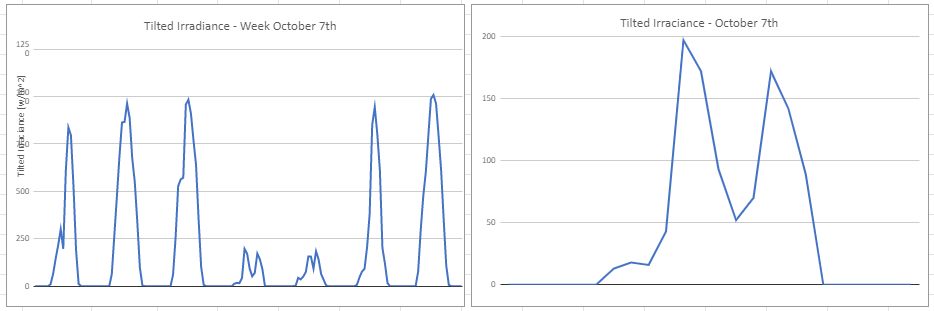
\includegraphics[width=0.5\textwidth]{inc/irr.png}
        \caption{Solar View tilted irradiance}
        \label{fig:solarview}
    \end{center}
\end{figure}

The historical data of track location, shows that on the day (October $7^{th}$) there is an expectation of significantly less nominal solar energy available. As shown \ref{fig:solarview} above the data expects a max of $200 W{\cdot}m^{-2}$ with significant midday dips. From this we can infer the very real possibly of heavy/intermittent cloud cover.

\begin{table}[h!]
    \begin{center}
        \begin{tabular}{|l|l|}
            \hline
            \multicolumn{2}{|c|}{\textbf{Average Irr race period 11:00 - 14:00}} \\ \hline
            \textit{Oct 7th}                   & \textit{Week}                   \\ \hline
            96.75                              & 612.61                          \\ \hline
        \end{tabular}
    \end{center}
\end{table}

To prevent drastically oversizing the final design and to ensure optimising for total costing of the system, we examined the average irradiance over the race time of both the week as a whole and of the day itself (see above). From this we proceeded forth with expectation that the panels may be operating at half their possible maximum output. This directly informed the amount of panels we chose in order to supply our energy requirements, especially due to possible large fluctuation erring on a robust rather than exactly matched system.

\subsection{Topology}

\begin{center}
    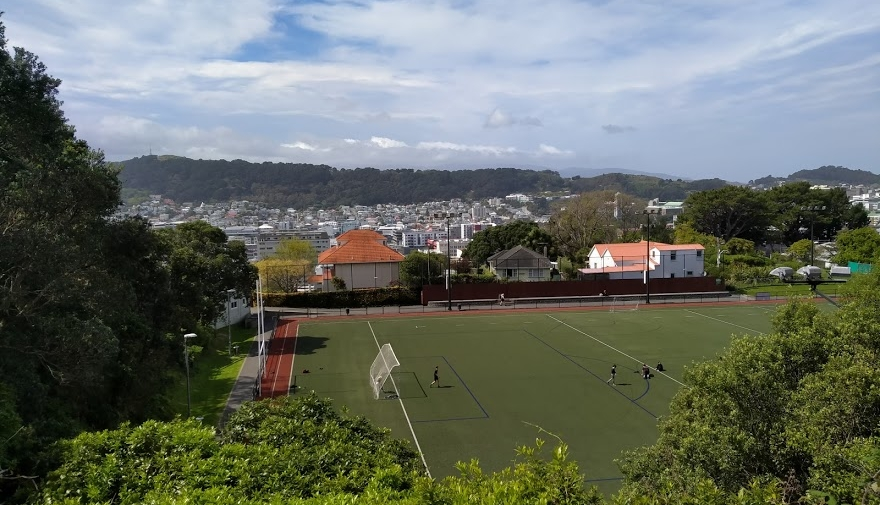
\includegraphics[width=0.5\textwidth]{inc/IMG20201006120746.jpg}
\end{center}

By visiting the site during the time on the week off the race, we were able to make an inspection of effects of shadows from building and trees. Seen above, the tree coverage of the northern tree line does not infringe on the section of field intended for solar collection, nor do any building. Therefore we can directly use the NIWA data under assumption that the only occlusion of direct sun we would experience would be cloud coverage.

\section{Race/Track Conditions}
\subsection{Description}
\begin{figure}[h!]
    \begin{center}
        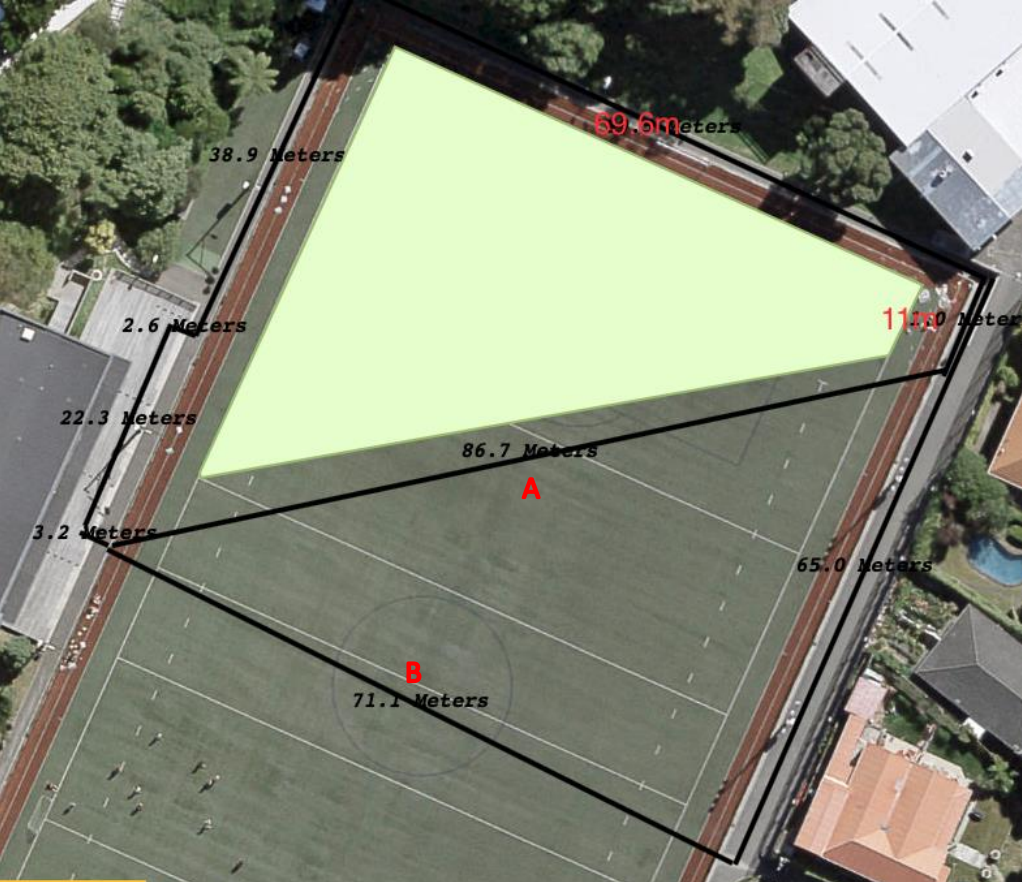
\includegraphics[width=0.42\textwidth]{inc/tracks.png}
        \caption{Track Options \cite{DANNYB}}
        \label{fig:routes}
    \end{center}
\end{figure}

The track as established consisted of two distinct course routes that were required to be chosen between. These are illustrated above [\ref{fig:routes}]: 

The first route, A, is roughly 234.3 meters and is roughly triangular.

The second , B, is $\approx 283.7$ meters but has the \textbf{possible} benefit of less distance on the turf.

The assumption that is required to be tested is that the current requirements of the 2 surface is of significant difference, ie higher on turf. Thus leading to a possible requirement of comparing trade off in potentially higher current draw to a shorter track.

\subsection{Testing}
To investigate the potential difference in motor performance, the testing procedure was to take one motor as a reference and perform set tasks while collected real-time data of current drawn from the battery.

We did this only for one motor to make observation to compare not necessarily the difference in motors but the general affect of surface and action on the power requirements of the platform.

\begin{figure}[h!]
    \begin{center}
        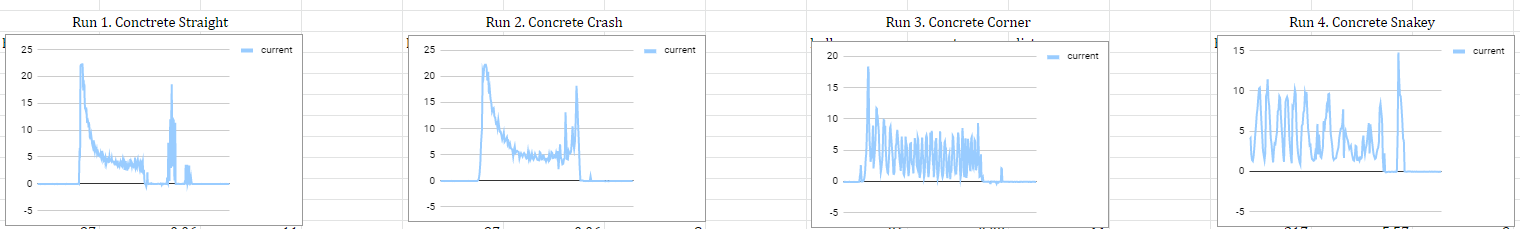
\includegraphics[width=\textwidth]{inc/contrete_behaviour.png}
        \caption{Concrete Performance}
        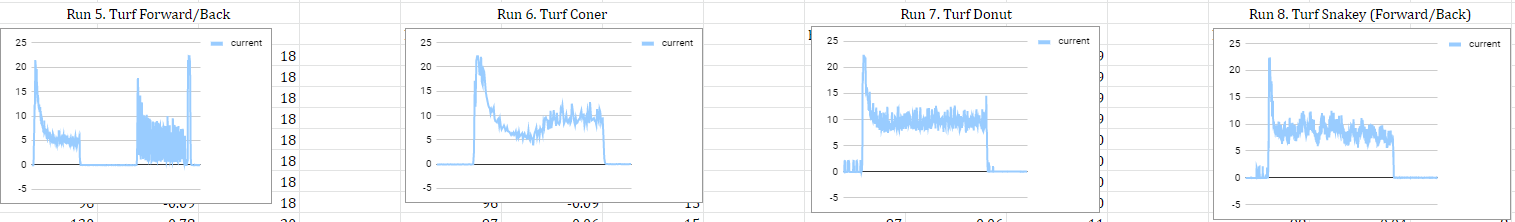
\includegraphics[width=\textwidth]{inc/turf_behaviour.png}
        \caption{Turf Performance}
    \end{center}
\end{figure}

We performed taking corners, from stand still acceleration and continuous turning on both surfaces build enough of an idea to compare.

From the data visualised above we observed a greater baseline current usage on the turf than the concrete, a significant up to 50\% greater current draw at times.

Behaviourally, it was observed that large acceleration spikes are consistent between the two surfaces, but due to the higher baseline of the turf the average current draw from a lot of turning and corner taking draw more current, more consistently.\\

Using this initial analysis, we concluded that being in more control of the car to increase the time at straight, constant speed and reduce accelerations would most likely increase the lifetime of the battery charge and that the trade off between reduced length and higher current draw would have to be further examined and made up for with other optimisations.



\section{Component Testing}
\subsection{Motors}
To characterise and compare available motor types and performance a 3m straight track was setup with a cardboard box and the end. The on board sensors recorded the current draw and distance from end to get a instantaneous current vs steepness of displacement graphs.

\begin{figure}[h!]
    \begin{center}
        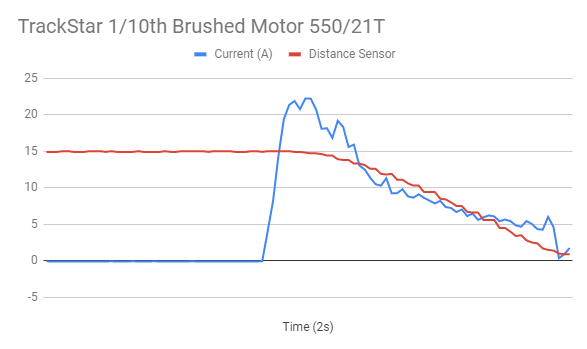
\includegraphics[width=0.3\textwidth]{inc/large_motor.png}
        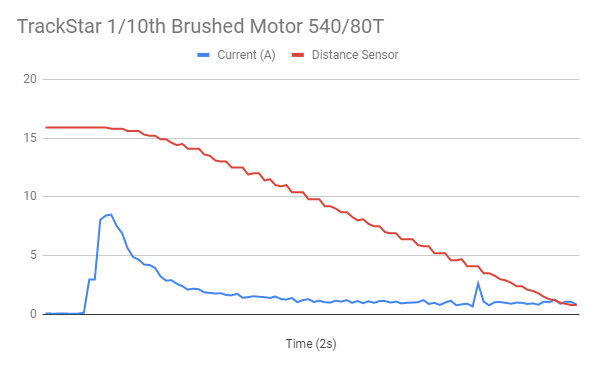
\includegraphics[width=0.3\textwidth]{inc/slow_motor.png}
        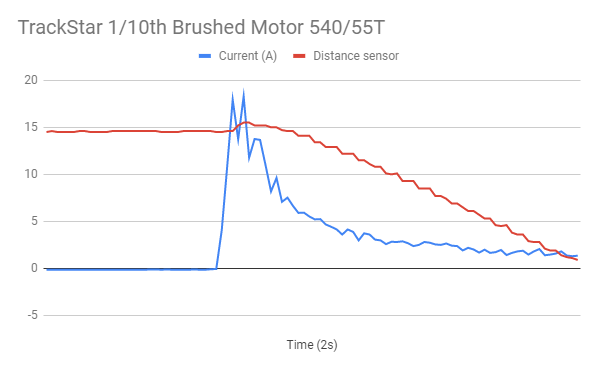
\includegraphics[width=0.3\textwidth]{inc/small_motor.png}
        \caption{Current and Displacement graphs}
    \end{center}
\end{figure}

From this data we observed that the highest rpm and largest motor, the 550/21T, had the highest speed and baseline current draw [10A - 5A] and the lowest rpm, 540/80T, was slowest with significantly lower current draw [3A - 1.5A], however it provided very high torque and due to the lower speed better handling. 

The 540/55T was not as drastically faster but still had a higher current requirement. In addition it difficult/impossible to mount correctly due to it small size so it was immediately discarded as a choice.

Two main considerations were taken in the selection between the 21T and the 80T:

\begin{itemize}
    \item Handling, ability to reduce random turning/crashing and other current spike inducing accelerations
    \item Current vs speed comparisons 
\end{itemize}

The 80T, due to much lower current spikes ($<$10 vs $>20$) and low speed was considered to be the most easily handled so we had to weigh a possible trade off in current/speed performance. The 21T is rated for 2.17 the rpm of the 80T and the tests confirm a very close to 2x distance coverage performance but the baseline current of the 80T was under two times that of the 21T so for this and the prior reason we chose the 80T.

\newpage
\subsection{Battery Capacity and Charge Time}
\begin{figure}[h!]
    \begin{center}
        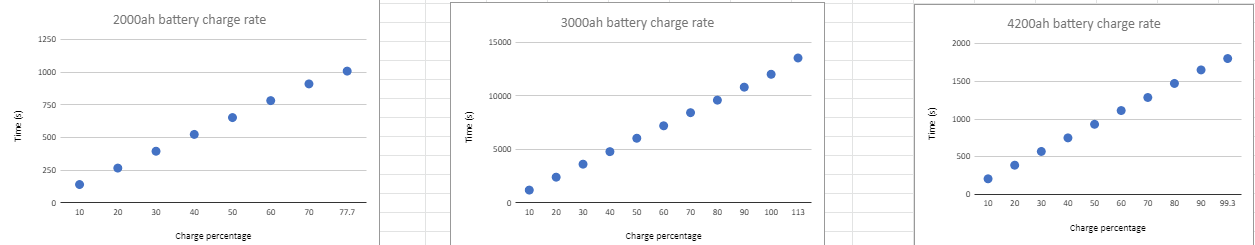
\includegraphics[width=0.5\textwidth]{inc/bat.png}
        \caption{Smart Battery Charging}
    \end{center}
\end{figure}

The use a smart charge controller, resulting in linear charge curves for every capacity at various charging currents, though the use of the charger incurs a 100 price tag that restricted flexibility. So we also explored the charging potential of a buck regulator.


\subsubsection*{Charger}
\begin{figure}[h!]
    \begin{center}
        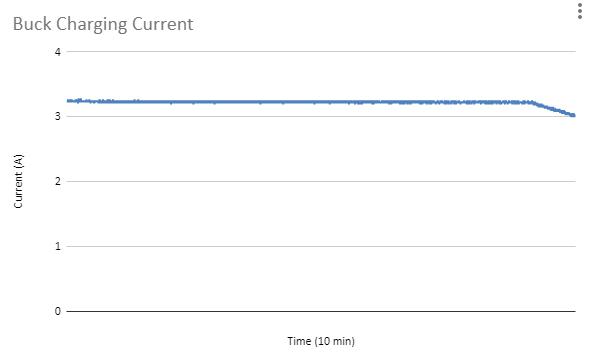
\includegraphics[width=0.5\textwidth]{inc/BUCK.png}
    \end{center}
\end{figure}

For the buck to be viable, we must be able to drive it with enough current to charge the battery high enough to operate the car for longer than the charge time.
For this reason we paired it with the MPPT and 12V lead-acid to ensure a 12V output. 

The test set the max output current of the buck to 4A at 9V and as shown above, resulted in a constant 3.24A charging current for almost 10mins. Further testing resulting in a (at 4A) 75\% charge in 10min from the buck.

From a test run, we measured that a the triangular track with the 80T motor consumed 239.99Wh, the test above resulting in ~5000Wh of "generated" energy so we estimated a very conservation 20 laps per 10mins of charge, which translate to roughly 30min of drive time (taken from a 92 second recorded test run).

For this reason, given that the charge station is capable to driving the buck at near test conditions, we selected the MPPT+Buck to recharge the battery.

\subsubsection*{Battery}
With the components tested for the car, we ran an observational test to test if we could run a reasonable run time with the smallest battery. We ran the 80T, with a fully charged 2000mAh battery around the track. 

We the battery lasted 30mins with only a 50\% discharge, and was able to take inclines both concrete and turf, so we decided to choose two 2000mAh so we could have 0 downtime.  

\newpage
\section{System Design}
\subsection{Charge Station}

Our max buck output power is 36W, based on the solar irradiance and conservative estimate of 50\% available output, we selected 6, 10W panels to drive the MPPT. These are wired in parallel 3 series pairs to give a output voltage or 24V and enable to MPPT to output around a 5A at good output.

This provided the best opportunity for the buck to outputting close to max current when connected to a depleted battery and enable us to charge in the 10min linear region per every hotswap.

\begin{center}
    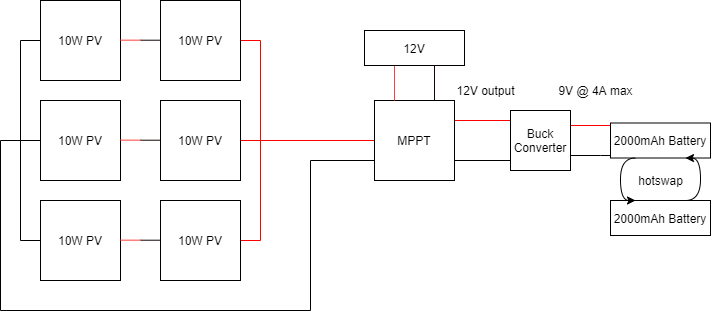
\includegraphics[width=0.5\textwidth]{inc/panels.png}
\end{center}

\subsection{Car}

Final car was the 80T, with a 2000mAh battery and second for hot swapping for zero downtime.

\begin{figure}[h!]
    \begin{center}
        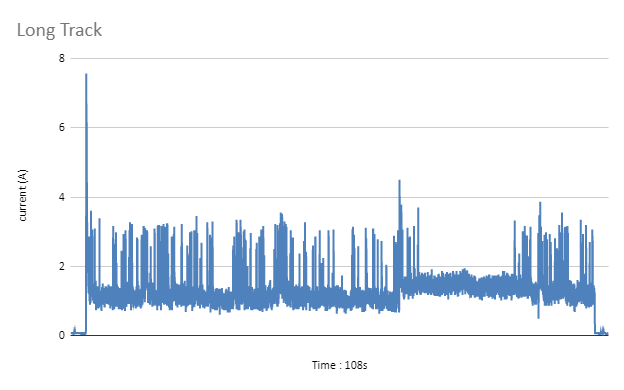
\includegraphics[width=0.3\textwidth]{inc/long_lap.png}
        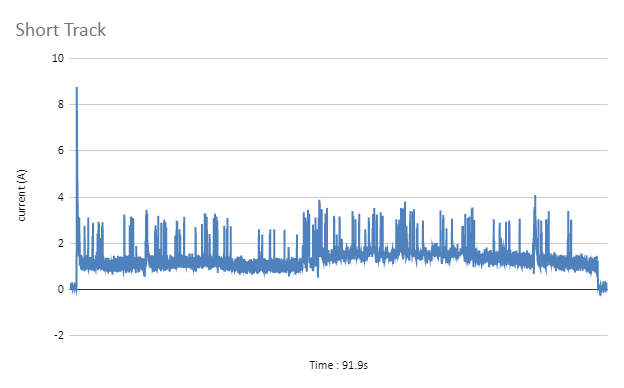
\includegraphics[width=0.3\textwidth]{inc/short_lap.png}
    \end{center}
\end{figure}

Using this platform we perform a final lap test for both tracks to decide on out final choice. As seen above the behavioural tests translate to the whole race and we see a higher base current draw for longer on the triangular track than that of the majority concrete track.

We took current measurement during this to calculate total energy usage per track.

$$Energy = V_{bat}{\cdot}A_{mean}*T$$

This was 265.7mWh for the long track and 239.99mWh for the short track, so we chose the short track.

\newpage
\section{Risk Analysis}
The 3 main risk contributors we aimed to mitigated in our design was:
\begin{itemize}
    \item Insufficient generation due to non-ideal conditions
    \item Downtime for charging
    \item Power spikes due to lack of control
\end{itemize}

The first 2 go hand in hand and lead as to oversize our production and storage (6 panels and 2 batteries) so be better suited to a greater range of operating conditions and make up for the cost increase by for example using a buck convertor.

We designed around the last point by using the slower more "torquey" motor.

\section{Budget}

\begin{table}[h!]
    \begin{center}        
    \begin{tabular}{|l|l|}
    \hline
    \multicolumn{2}{|c|}{\textbf{Team ECO Budget}}            \\ \hline
    6 x 12V 10W Polycrystalline solar panel & 285.42 \\ \hline
    buck                                    & 12.39  \\ \hline
    MPPT + 12V bat                          & 86.85  \\ \hline
    2 x NiMH battery 2000mAh                & 154.44 \\ \hline
    TrackStar 1/10th Brushed Motor 540/80T  & 14.04  \\ \hline
    \textbf{total}                          & \textbf{553.14} \\ \hline
    \end{tabular}
    \end{center}
    \end{table}
\section{Conclusion}
All in all, we were able to utilise simulated lab tested, on site test runs, direct data collection and historical datasets to drive our analysis of both the availability of the generation resource but also the consumption. This was then used to optimise for a balance in cost, performance and robustness by matching the generation to the requirement load and its dynamics.

This may have been in the realm of RC cars but it make use of skills and techniques developed on household based systems and the growth in knowledge and experience is directly transferable back into the design of any renewable based stand-alone generation solution.

\bibliography{ref}
\bibliographystyle{IEEEtran}
\end{document}
